\documentclass{article}
\usepackage[utf8]{inputenc}

\title{legendre functions}
\author{Alex}
\date{September 2020}

\usepackage{natbib}
\usepackage{graphicx}

\begin{document}

\maketitle

\section{Introduction}
There is a theory which states that if ever anyone discovers exactly what the Universe is for and why it is here, it will instantly disappear and be replaced by something even more bizarre and inexplicable.
There is another theory which states that this has already happened.

\begin{quote}
The Encyclopedia Galactica defines a robot as a mechanical apparatus designed to do the work of a man. The marketing division of the Sirius Cybernetics Corporation defines a robot as `Your Plastic Pal Who's Fun to Be With.` The Hitchhiker's Guide to the Galaxy defines the marketing devision of the Sirius Cybernetic Corporation as `a bunch of mindless jerks who'll be the first against the wall when the revolution comes.`
\end{quote}

\begin{figure}[h!]
\centering
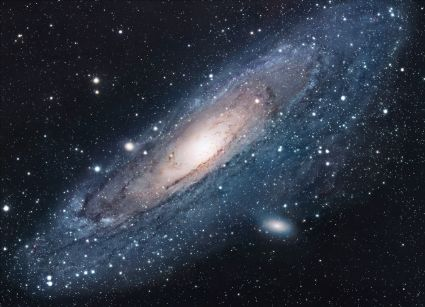
\includegraphics[scale=1.7]{universe}
\caption{The Universe}
\label{fig:universe}
\end{figure}

\section{Conclusion}
``I always thought something was fundamentally wrong with the universe'' \citep{adams1995hitchhiker}

\bibliographystyle{plain}
\bibliography{references}
\end{document}
